\section{Konzept}

\begin{figure}[H]
  \begin{center}
    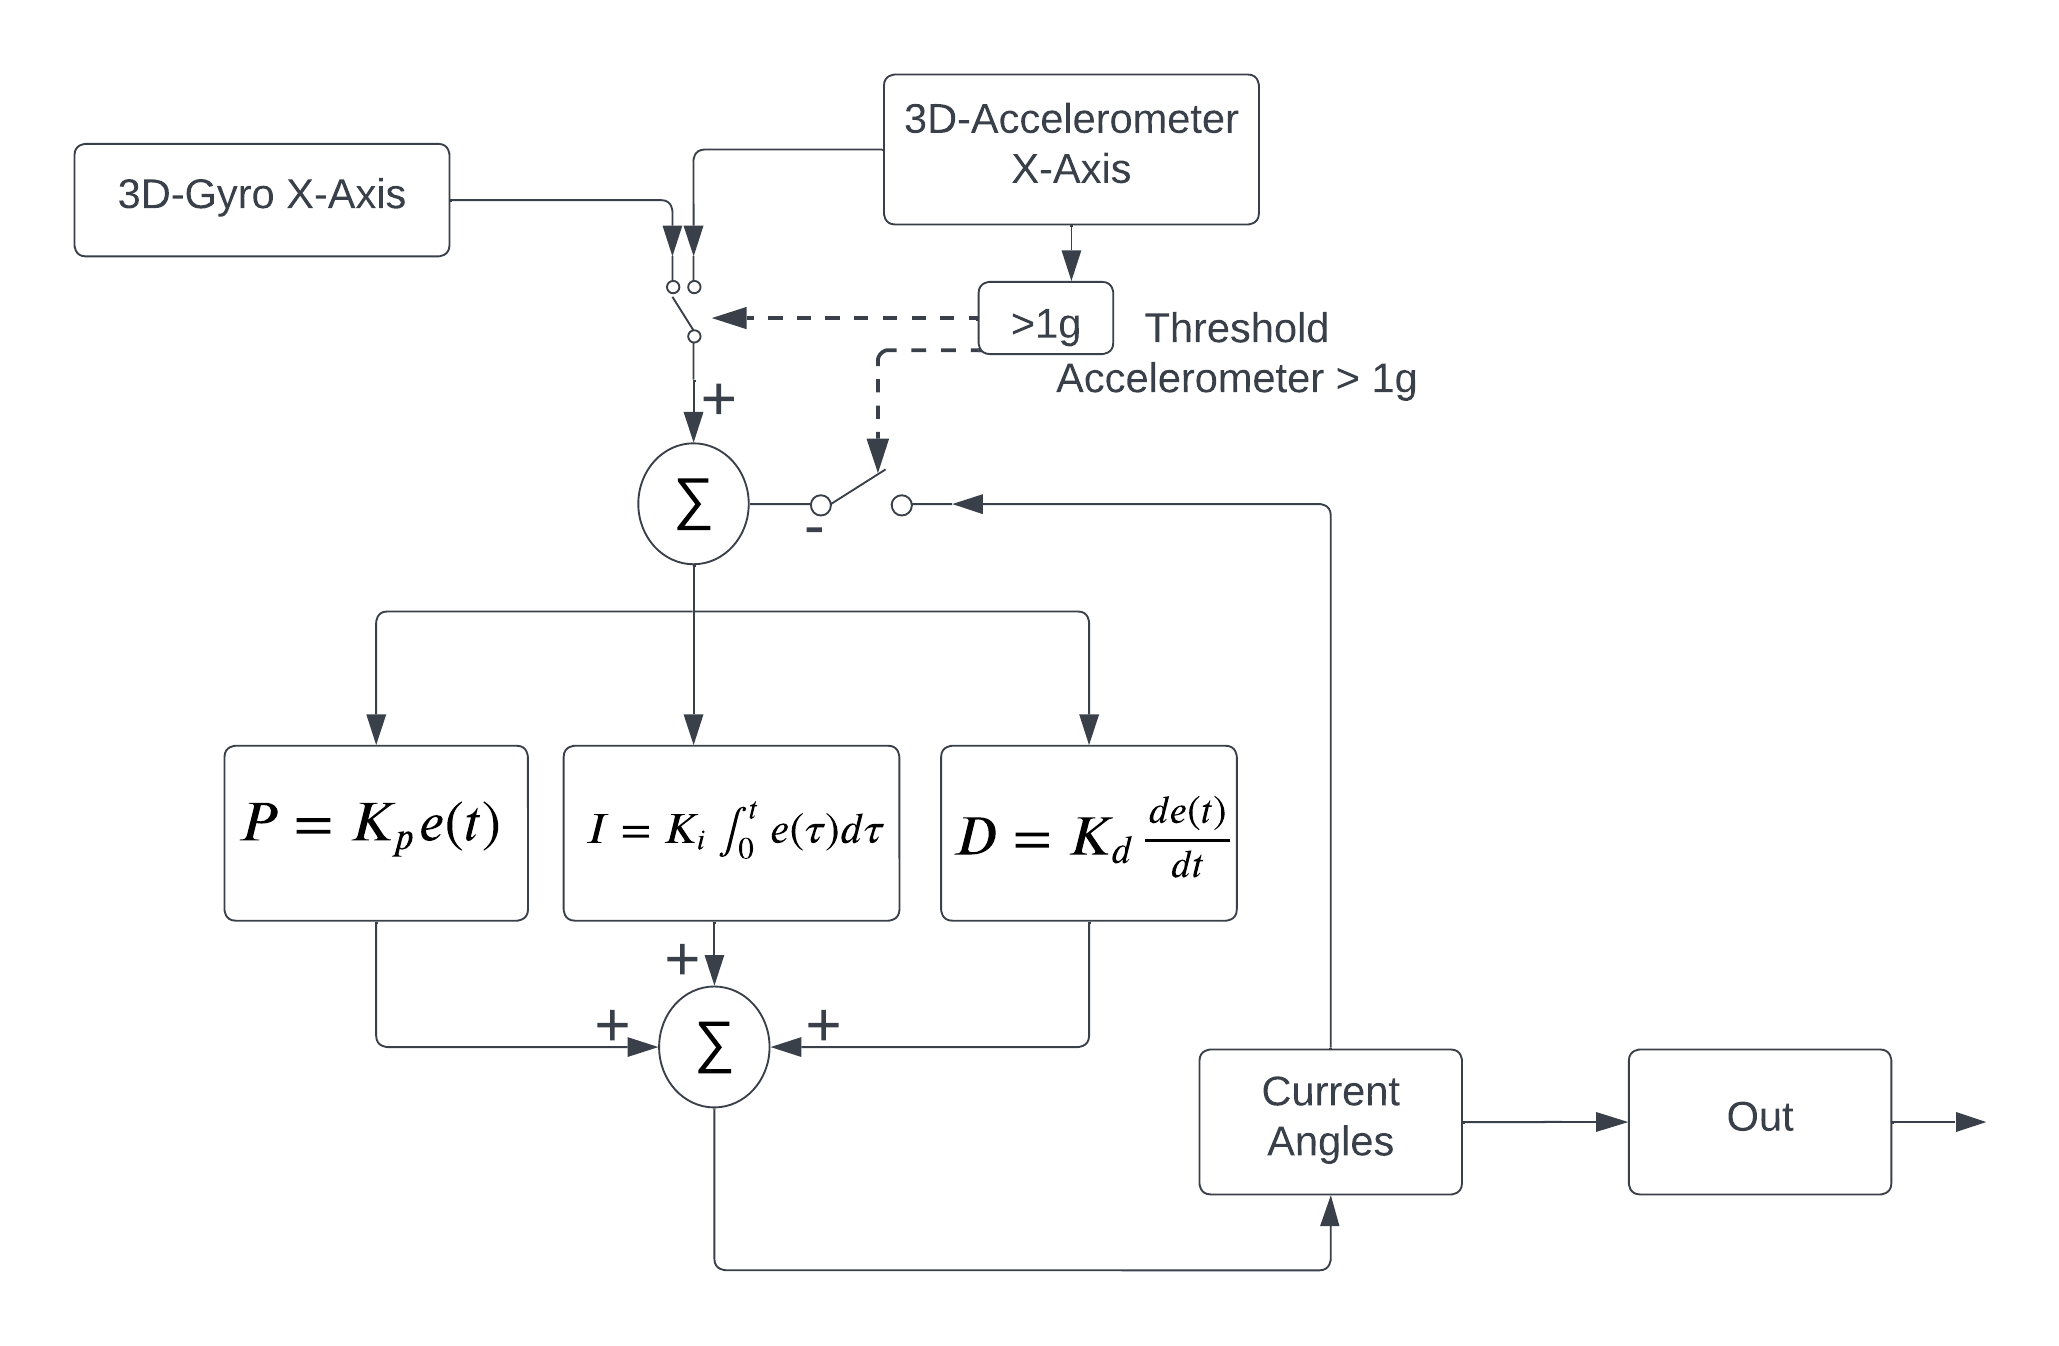
\includegraphics[width=1\linewidth]{content/images/PID_Loop.png}
    \caption{PID Loop}
  \end{center}
\end{figure}

\subsection{UseCase}
\begin{figure}[H]
  \begin{center}
    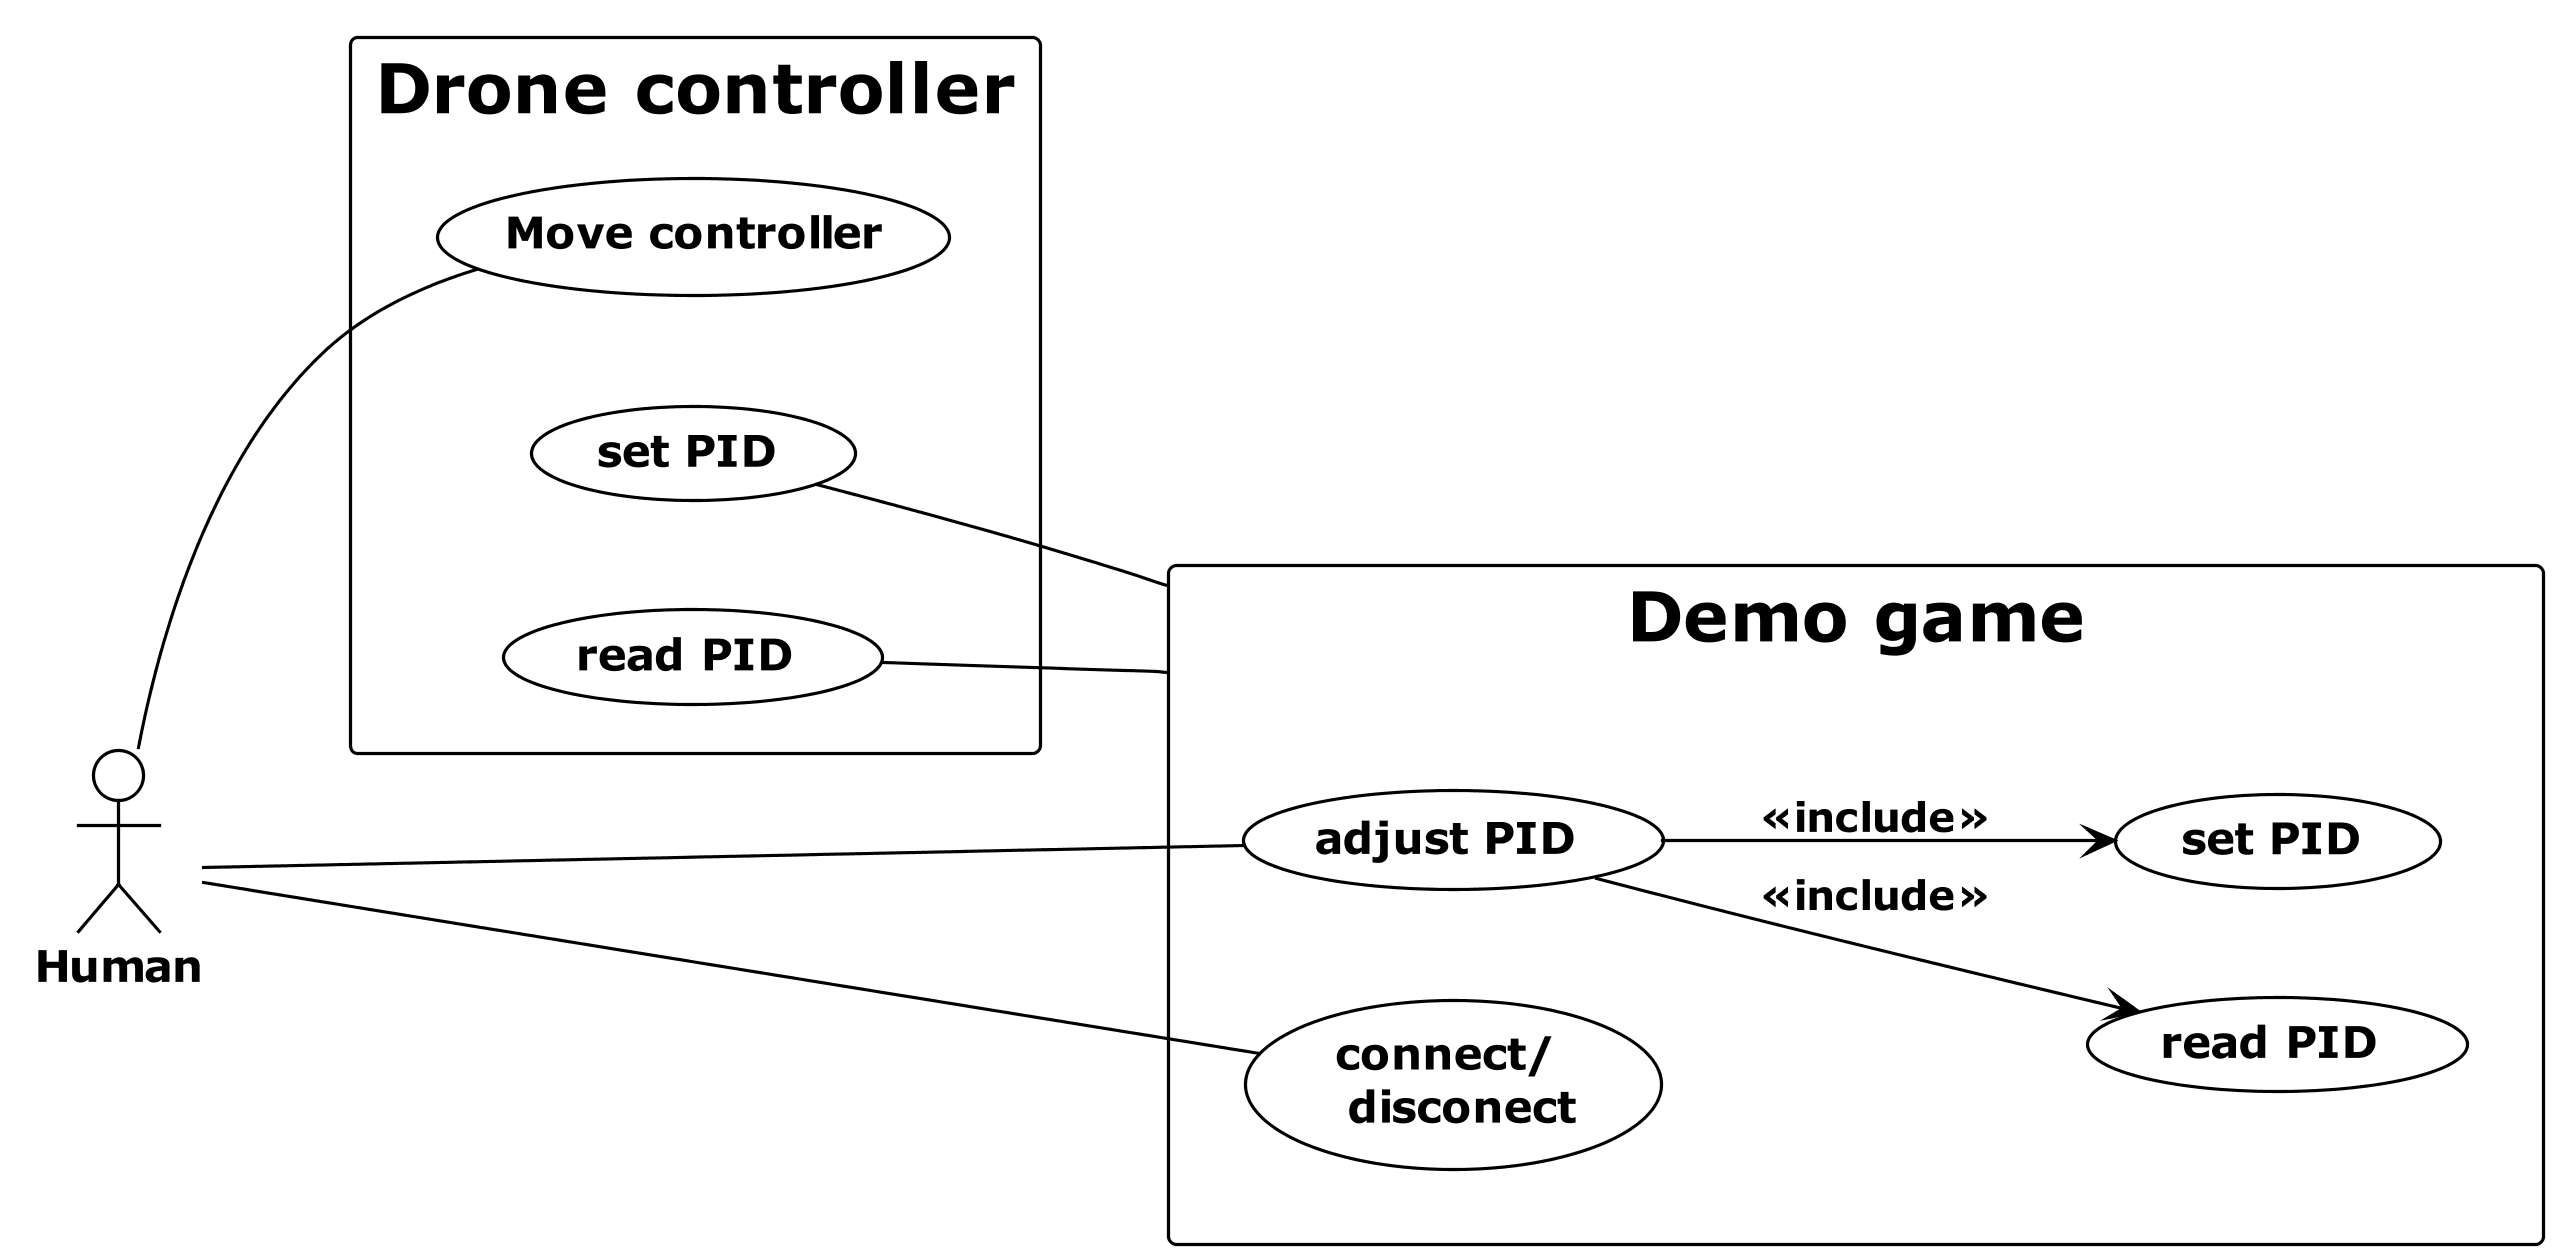
\includegraphics[width=0.9\linewidth]{content/diagrams/out/usecase/sendAngles.png}
    \caption{Send angles}
  \end{center}
\end{figure}

\subsection{Sequenzdiagramme}
\begin{figure}[H]
  \begin{center}
    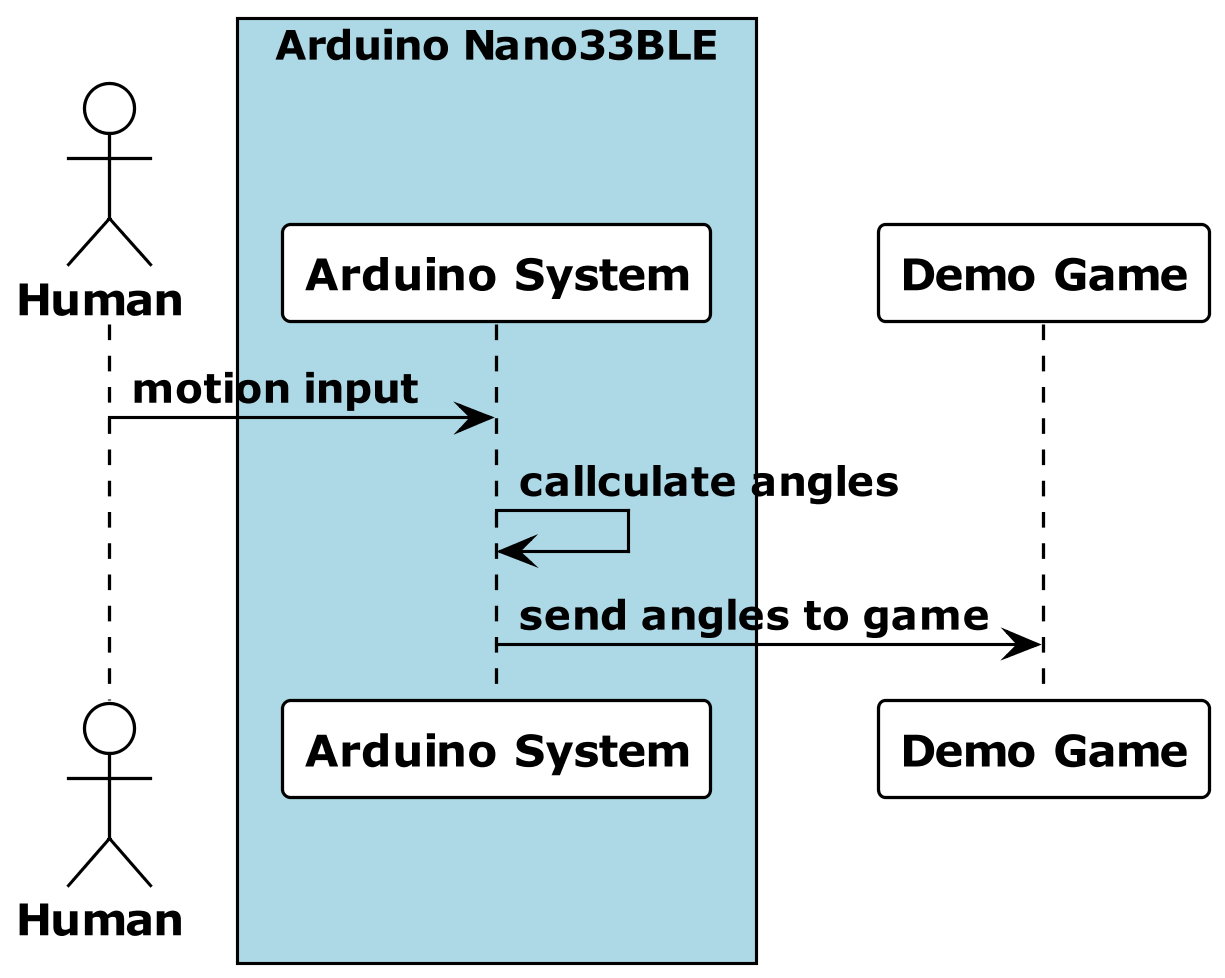
\includegraphics[width=0.7\linewidth]{content/diagrams/out/sequence/system.png}
    \caption{System}
  \end{center}
\end{figure}

\begin{figure}[H]
  \begin{center}
    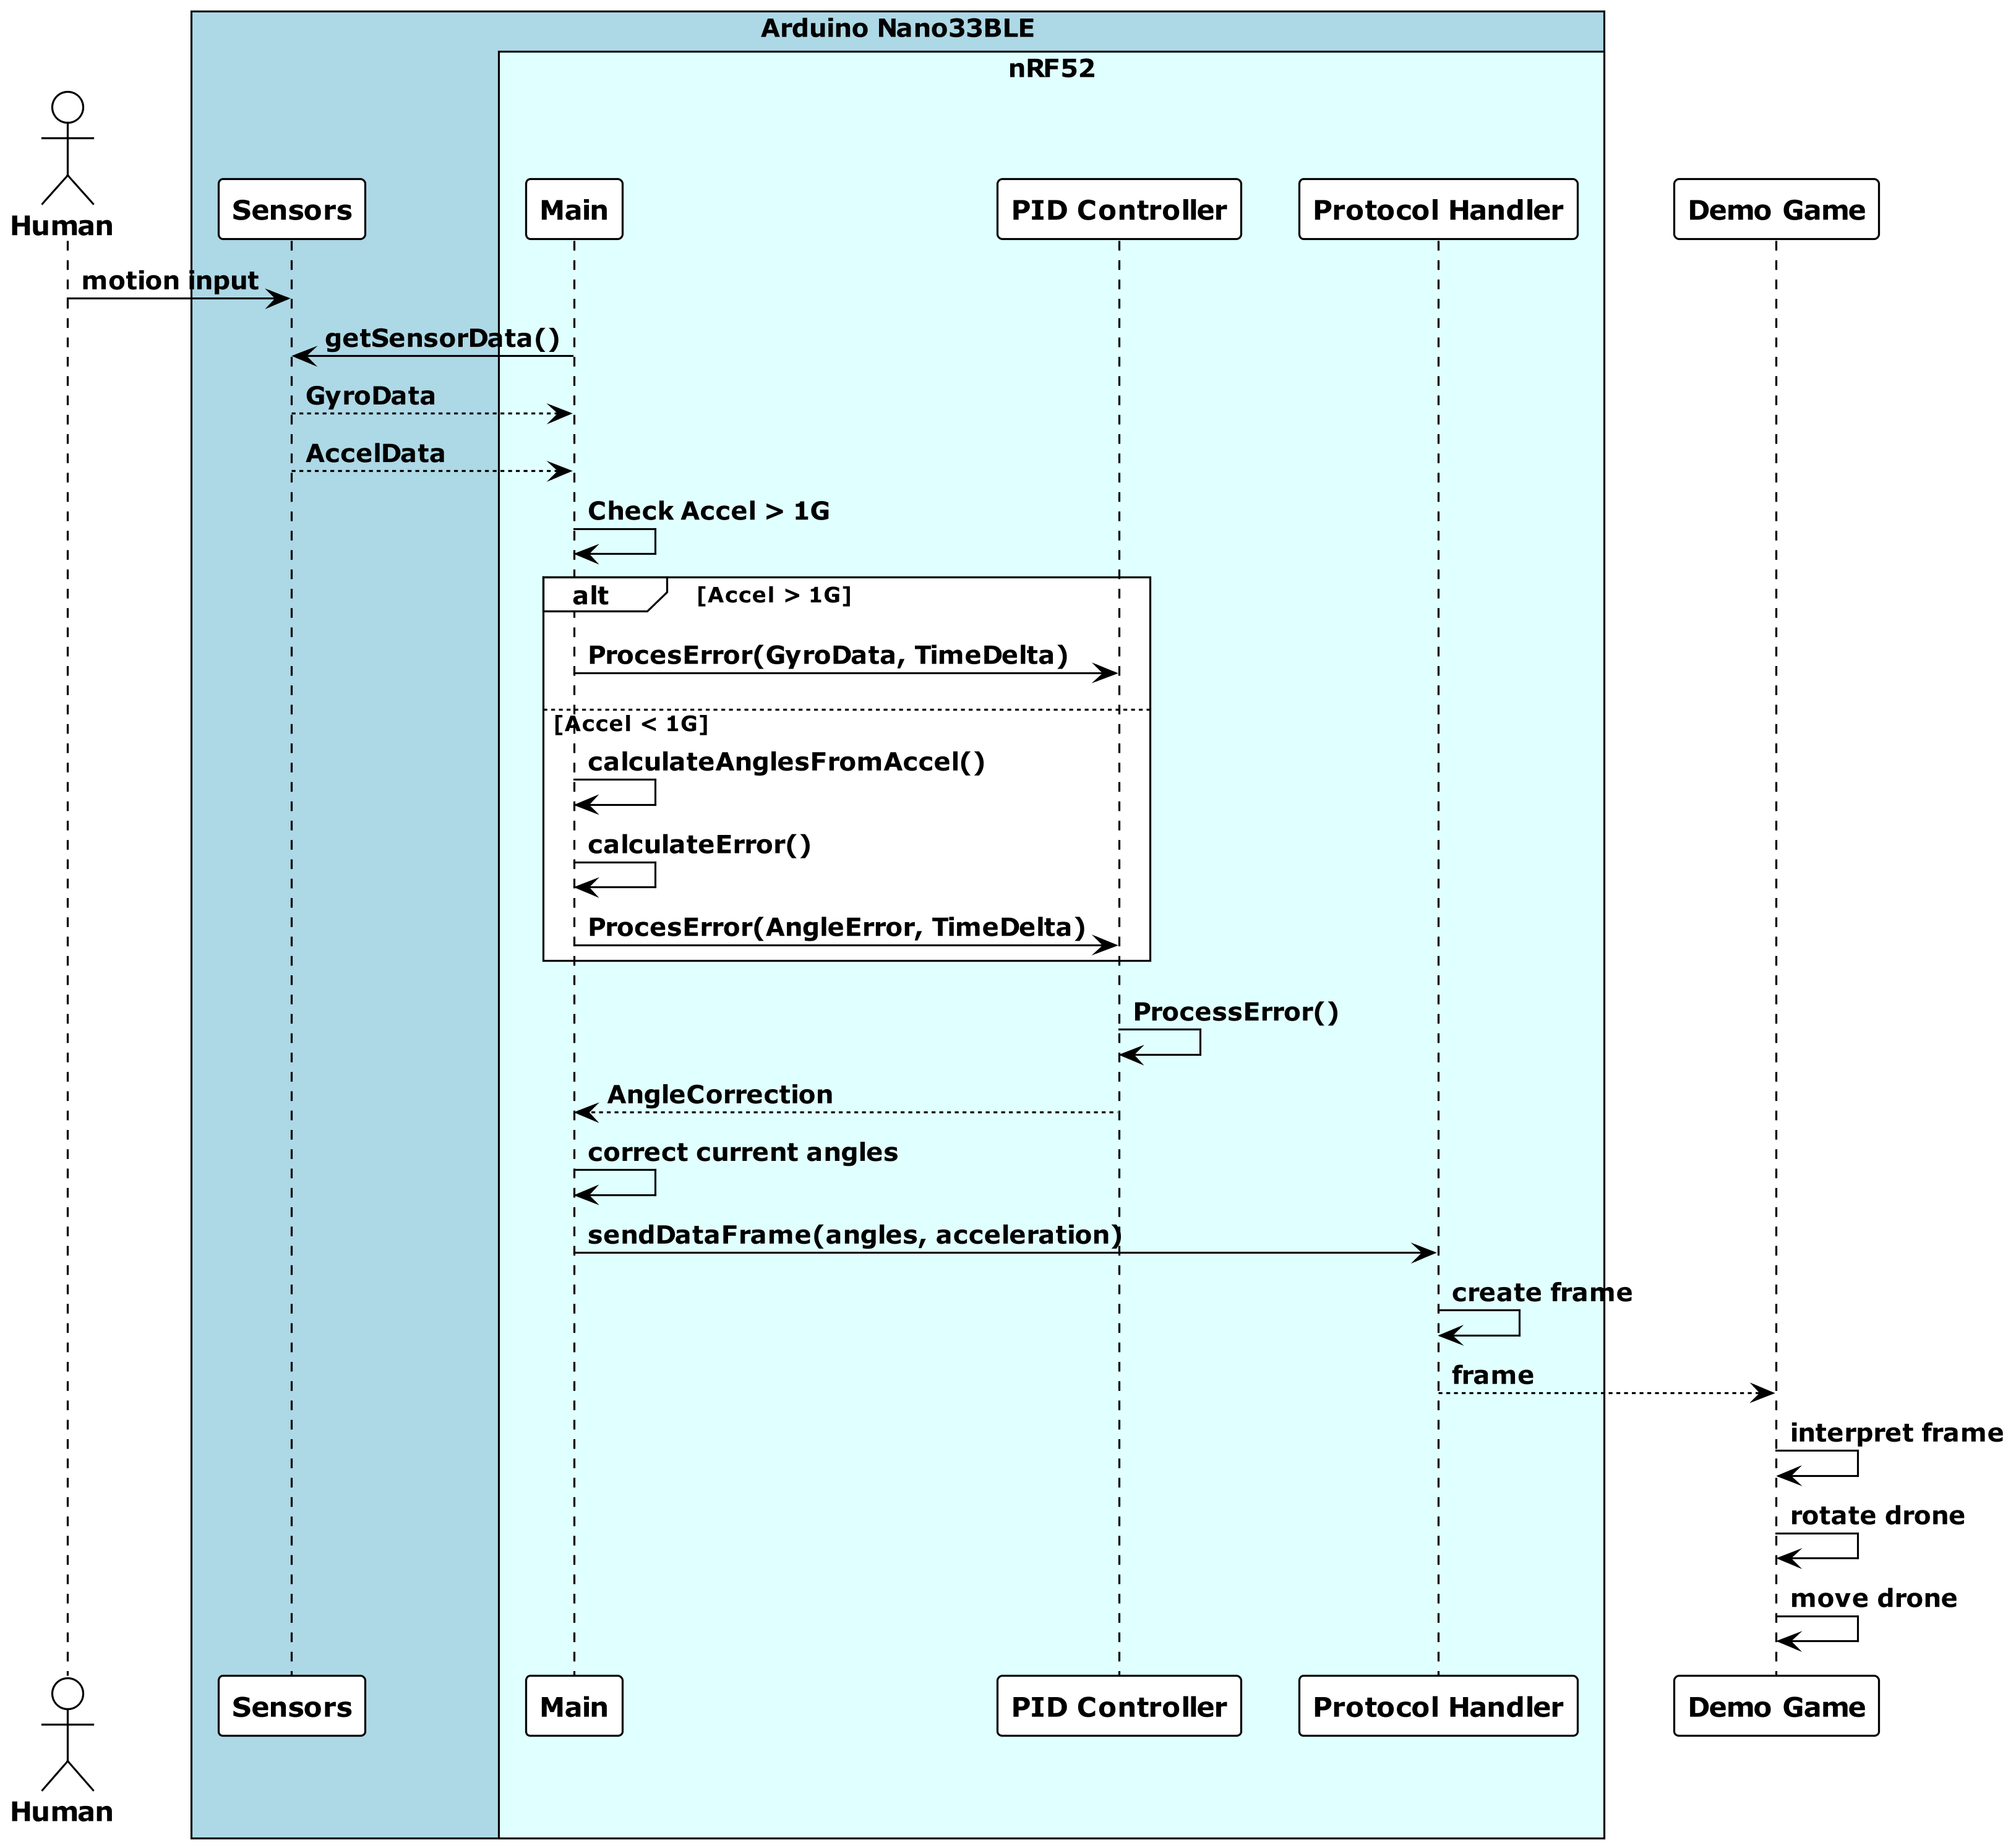
\includegraphics[width=1\linewidth]{content/diagrams/out/sequence/moveController.png}
    \caption{Move controller}
  \end{center}
\end{figure}

\subsection{Klassendiagramm}
\begin{figure}[H]
  \begin{center}
    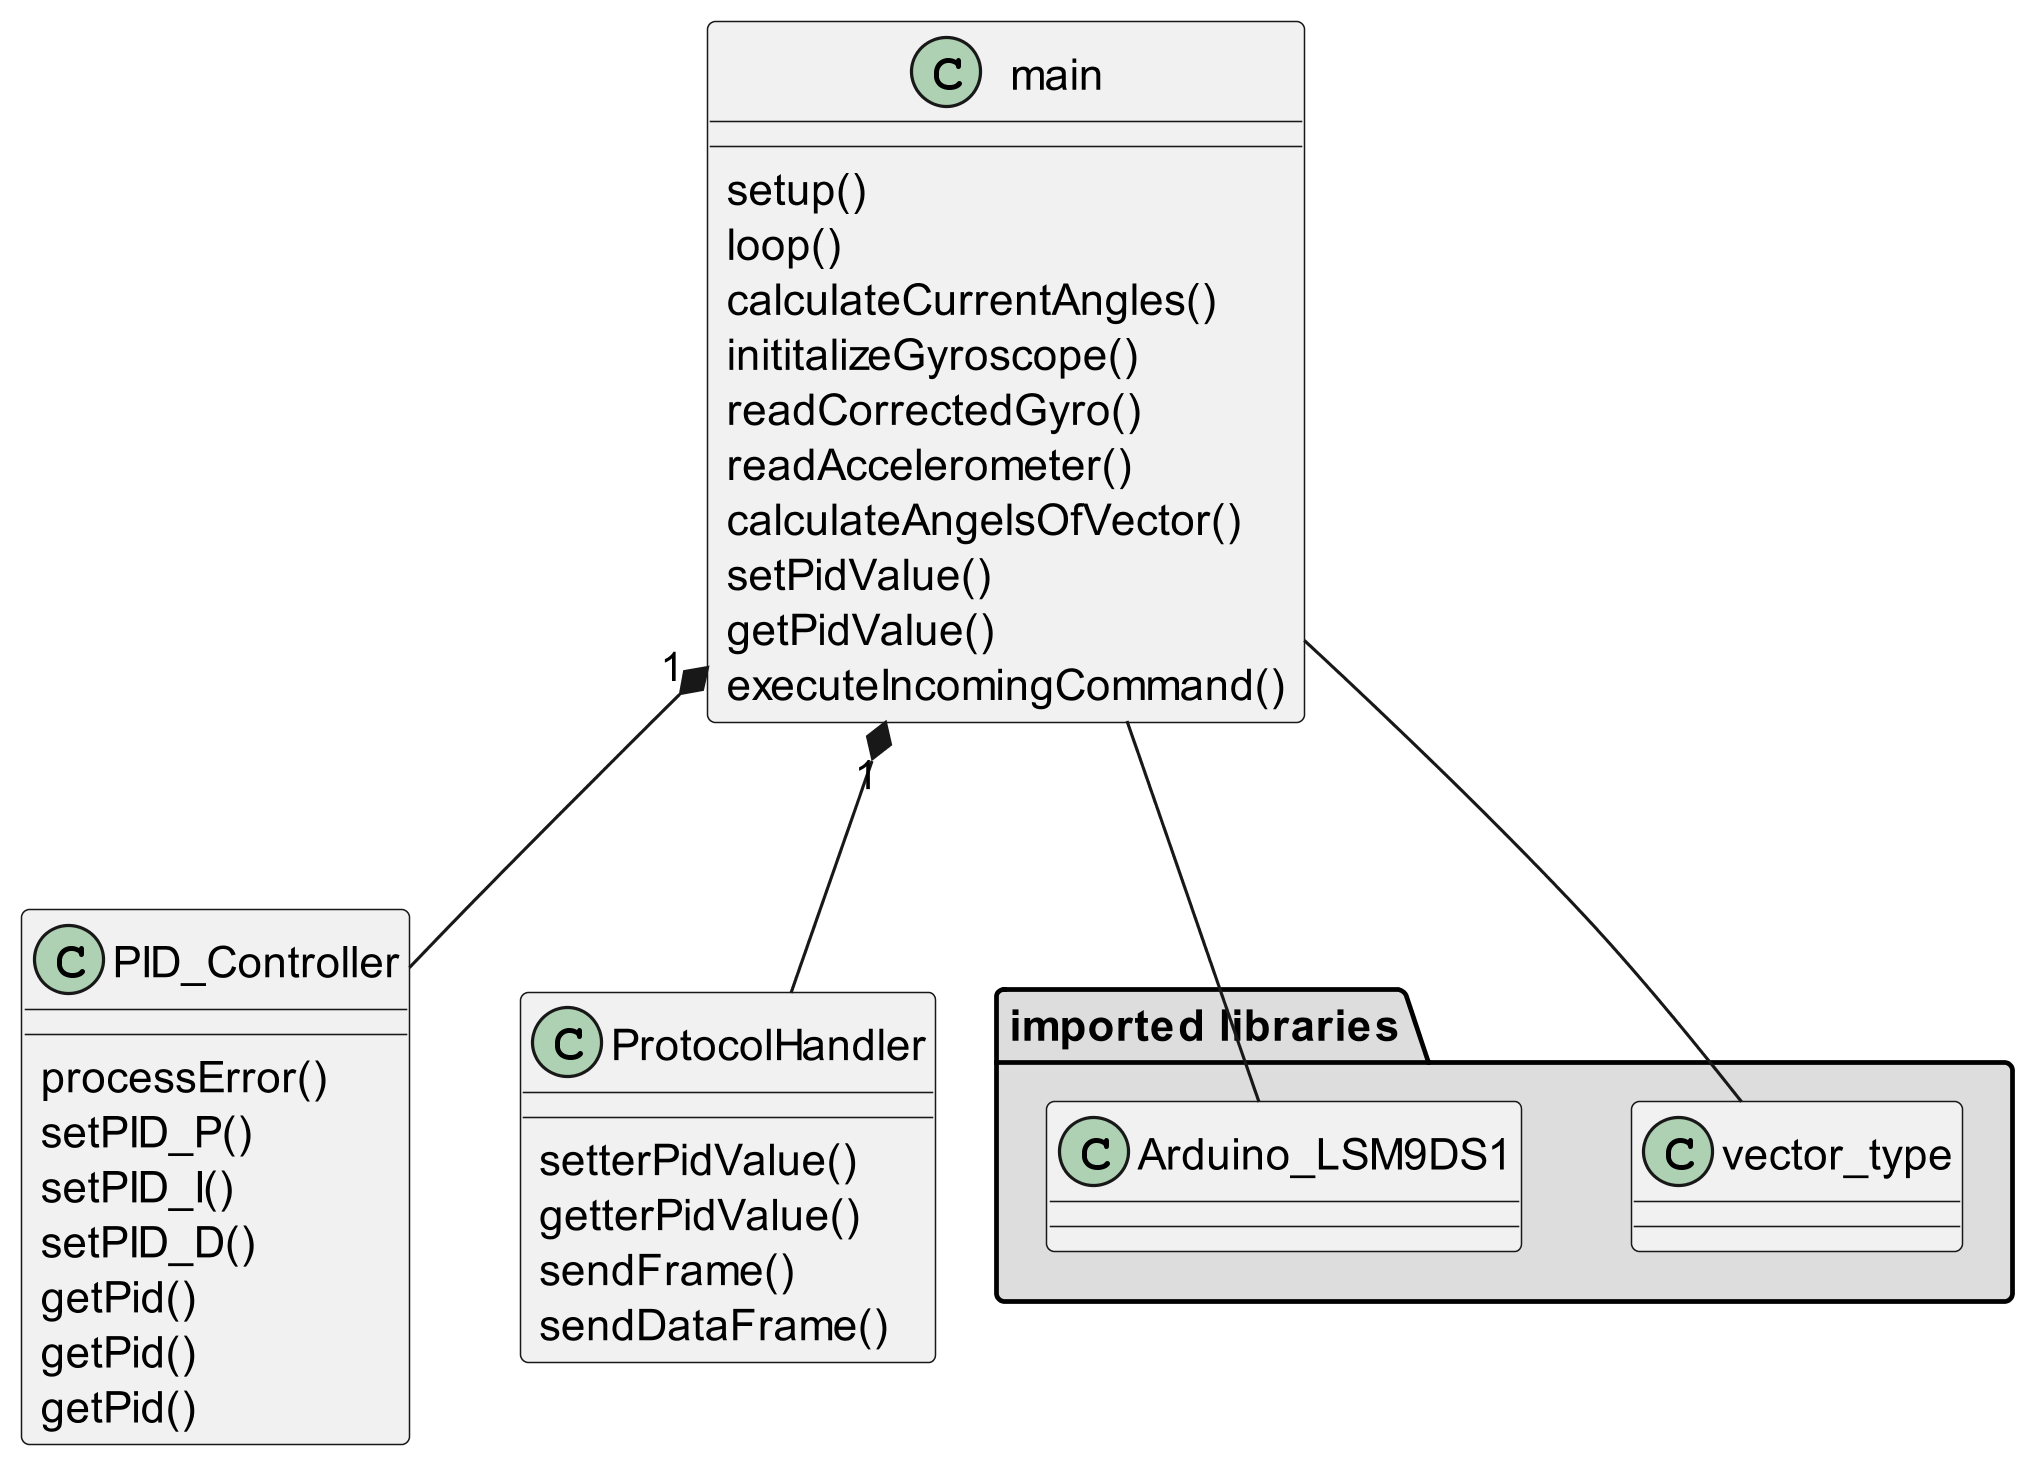
\includegraphics[width=0.8\linewidth]{content/diagrams/out/class/classdiagram.png}
    \caption{Klassendiagramm}
  \end{center}
\end{figure}

\subsection{Beschreibung der Klassen und Funktionen}
In diesem Kapitel werden die benutzten Klassen und deren Funktion kurz beschrieben.
\subsubsection{''main'' Klasse}
Die ''main'' Klasse ist die hauptklasse welche alle anderen Klassen Importiert. Hier befindet sich ebenfalls die setup() Funktion und die loop() Funktion welche im Arduino vorgeben sind.

\begin{table}[H]
  \centering
  \settowidth\tymin{executeIncomingCommand()}
  \setlength\extrarowheight{2pt}
  \begin{tabulary}{1.0\textwidth}{|L|L|}
    \hline
    \textbf{Funktion} &
    \textbf{Beschreibung}\\
    \hline
    setup() &
    Setupfunktion des Arduino. Wird ausgeführt wenn der Arduino gestartet wird.\\
    \hline
    loop() &
    Der Loop ist eine Endlosschleife, der nach jedem Durchlauf erneut aufgerufen wird.\\
    \hline
    initializeGyroscope() &
    Mit dieser Funktion wird das Gyroskop beim einschalten initialisiert und kalibriert.\\
    \hline
    calculateCurrentAngles() &
    \\
    \hline
    readCorrectetGyro() &
    \\
    \hline
    readAcceletometer() &
    \\
    \hline
    calculateAnglesOfVector() &
    \\
    \hline
    executeIncomingCommand() &
    Diese Funktion wertet den eingegangenen Befehl aus und führt anschliessend die entsprechende Funktion aus.\\
    \hline
    setPidValue() &
    Wird aus executeIncomingCommand() aufgerufen und setzt die eingegangenen PID-Werte über den PID Controller.\\
    \hline
    getPidValue() &
    Wird aus executeIncomingCommand() aufgerufen und sendet die angeforderten PID Werte zurück.\\
    \hline
  \end{tabulary}
  \caption{Beschreibung der ''main'' Klasse}
\end{table}

\subsubsection{PID Controller}
TODO
\begin{table}[H]
  \centering
  \settowidth\tymin{processError()}
  \setlength\extrarowheight{2pt}
  \begin{tabulary}{1.0\textwidth}{|L|L|}
    \hline
    \textbf{Funktion} &
    \textbf{Beschreibung}\\
    \hline
    processError() & \\
    \hline
    setPID\_() & Setzt den eingehenden Wert einsprechend für P, I oder D. \\
    \hline
    getPID\_() & Sendet den aktuellen P,I oder D- Wert zurück.\\
    \hline
  \end{tabulary}
  \caption{Beschreibung PIDController}
\end{table}


\subsubsection{ProtocolHandler}
Mit dem ProtocolHandler wird das sende und empfangsprotokoll zum Steuern des Gamedemos kontrolliert.
\begin{table}[H]
  \centering
  \settowidth\tymin{sendPIDToSerial()}
  \setlength\extrarowheight{2pt}
  \begin{tabulary}{1.0\textwidth}{|L|L|}
    \hline
    \textbf{Funktion} &
    \textbf{Beschreibung}\\
    \hline
    setterPidValue() &
    Wertet den eingegangen Befehl zum setzen des PID-Werts aus und führt dann die entsprechende Funktion über den PIDController aus. \\
    \hline
    getterPidValue() &
    Wertet den eingegangen Befehl zum lesen des Aktuellen PID-Werts aus, holt sich den wert über den PIDController und sendet diesen über die Funktion sendPIDToSerial() zurück.\\
    \hline
    sendPIDToSerial() & 
    Wird durch getterPIDValue() aufgerufen und sendet PID-Wert über Serial.println() als string zurück.\\
    \hline
    sendDataFrame() &
    Wird durch den loop() aufgerufen und sendet die berechneten Gyro- und Beschleunigungsdaten Serial.println() als string an das Demo-Game.\\
    \hline
  \end{tabulary}
  \caption{Beschreibung ProtocolHandler}
\end{table}

\newpage